\documentclass[12pt,letterpaper]{article}

\usepackage[utf8]{inputenc}

% Page layout
%\usepackage[a4paper]{geometry}
%\geometry{hscale=0.75,vscale=0.75,centering}
\usepackage{fullpage}

% Include images
\usepackage{graphicx}

% Math equations
\usepackage{amsmath}
\usepackage{amssymb}
\usepackage[french]{babel}

% Include Matlab code with accents
\usepackage{listingsutf8}
\lstset{inputencoding=utf8/latin1}
\usepackage[framed]{mcode}


\begin{document}

    \begin{titlepage}
    \vspace*{3.5cm}
    \begin{center} 
        \LARGE{ \textbf{INF6800 - Conception geométrique assistée par ordinateur} }\\[1cm]
        \Large{Travail pratique numéro 1.}\\
        \normalsize{05/02/2014}\\[1cm]
        \normalsize{ \textit{Anis Benyoub} }
    	\begin{figure}[ht]
	\centering
	\end{figure}
    \end{center}
    
\end{titlepage}
     
	\newpage
	
    \section{Infos:}
	J'ai rendu les fichiers ainsi que le makefile mais pas les fichiers de projet visual studio.

    \section{Courbes d'Hermite:}
	\setlength{\parindent}{1cm}

	Dans cette partie j'ai implémenté 3 techniques de resolution pour la résolution des équations des courbes d'Hermite. Cette resolution est équivalente à la résolution d'un système A.x = b.\\
	Dans le premier cas (tangeantes imposées), la resolution du système est équivalent à la resolution d'un système tridiagonal. Je me suis grandement inspire de \"Numerical recipes in C\" http://www.haoli.org/nr/bookcpdf/c2-4.pdf pour l'algorithme. Je l'ai appliqué une fois par point (au lieu de l'appliquer une fois pour chaque coordonnée).\\
	Voici le resultat visuel que donne cette partie:
\begin{figure}[h!]
	\centering
	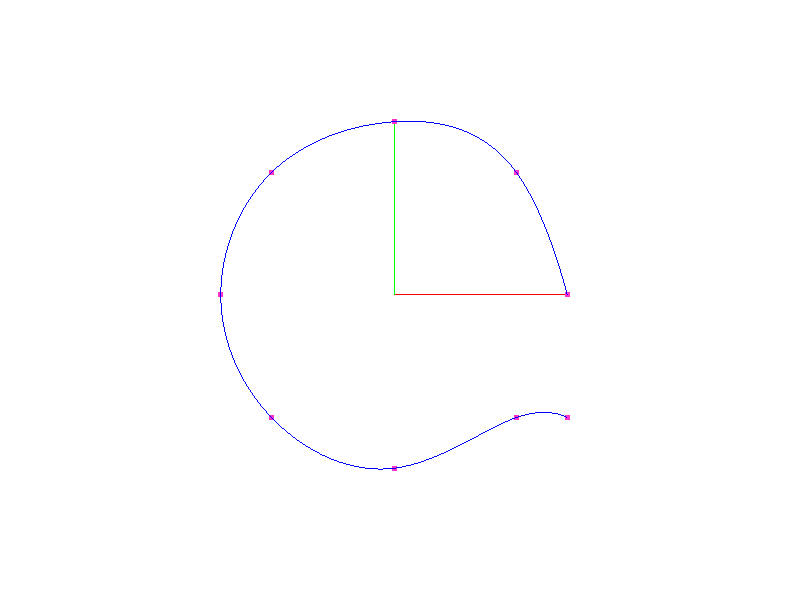
\includegraphics[scale=0.3]{images/imposedtang.png}
	\caption{\textit{Rendu de la scène pour le cas des tangeantes imposées.}}
\end{figure}
	
	Le deuxième cas (courbure imposée), la resolution du système est aussi équivalent à la resolution d'un système tridiagonal, les matrices A et B changent simplement car les contraintes du système changent.\\
	Voici le resultat visuel que donne cette partie:
	\newpage
\begin{figure}[h!]
	\centering
	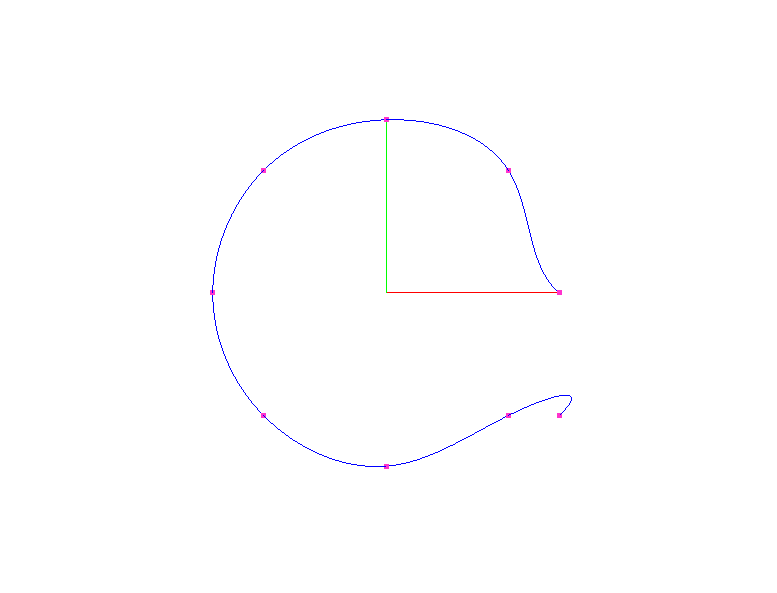
\includegraphics[scale=0.3]{images/imposedcurv.png}
	\caption{\textit{Rendu de la scène pour le cas des courbures imposées.}}
\end{figure}
	Le troisème cas de la courbure nulle est exactement celui de la courbure imposée mais avec des valeurs nulles.
	Voici le resultat visuel que donne cette partie:
\begin{figure}[h!]
	\centering
	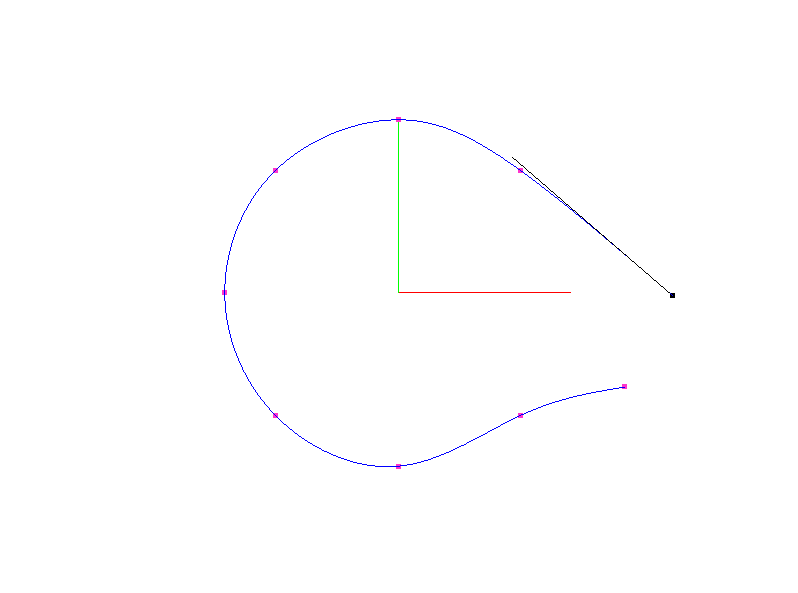
\includegraphics[scale=0.3]{images/nilcurv.png}
	\caption{\textit{Rendu de la scène pour le cas des courbures nulle.}}
\end{figure}

	Le dernier cas (\"courbure fermée\"), le système est toujours un système matriciel, simplement on passe dans un cas de système cyclique tridiagonal.\\
	Je me suis inspiré de l'algorithme de numerical recipes in C http://www.haoli.org/nr/bookcpdf/c2-7.pdf.\\\\
	De la même manière que pour les autres examples, le traitement se fait une fois par point au lieu d'une fois par coordonnée. L'algorithme transforme le système cyclique en système non cyclique puis le résoud. On retransforme les resultats pour les faire correspondre à nos besoins.\\\\
    Voici le resultat visuel que donne cette partie:
    \begin{figure}[h!]
	\centering
	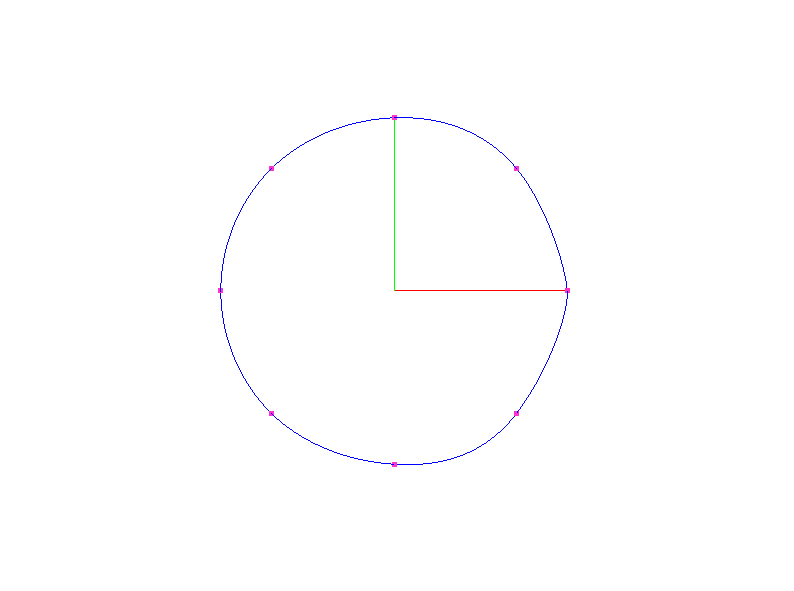
\includegraphics[scale=0.3]{images/closedcurv.png}
	\caption{\textit{Rendu de la scène pour le cas des courbures nulle.}}
	\end{figure}

    \section{Courbes de bezier:}
	\setlength{\parindent}{1cm}
    Cette partie est beaucoup simple que la première partie. J'ai choisi l'implémentation récursive de l'algorithme. Une implémentation itérative est tout a fait possible.\\
    Voici le resultat visuel que donne cette partie:
    \begin{figure}[h!]
	\centering
	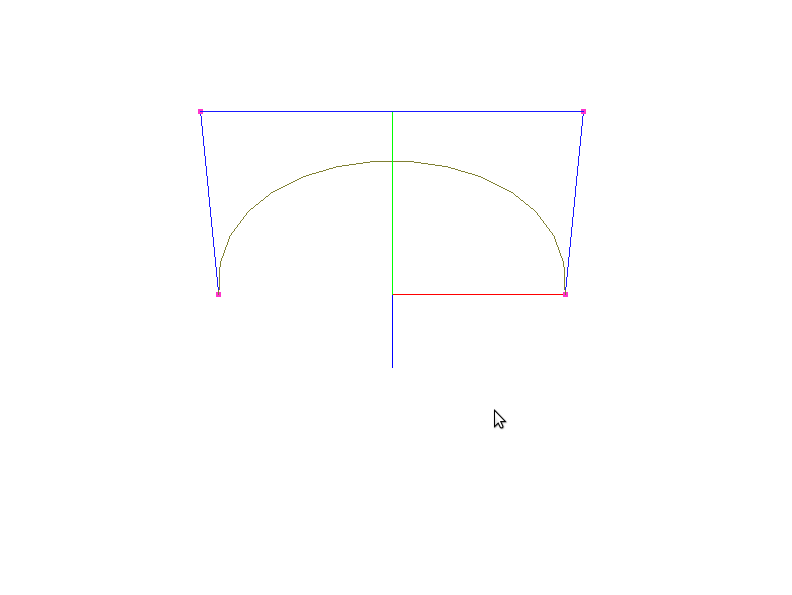
\includegraphics[scale=0.3]{images/bezier.png}
	\caption{\textit{Courbe de bezier en gris pour la courbe en bleu.}}
	\end{figure}

\end{document}

